\documentclass[12pt]{article}
\usepackage{amsmath}
\usepackage{amssymb}
\usepackage{amsthm}
\usepackage[font=small,margin=3em,skip=0em]{caption}
\usepackage{float}
\usepackage[T1]{fontenc}
\usepackage{fullpage}
\usepackage[hidelinks]{hyperref}
\usepackage{inconsolata}
\usepackage{listings}
\usepackage{mathdots}
\usepackage{mathpartir}
\usepackage{turnstile}
\usepackage{pst-node}
\usepackage{tikz}
\usepackage{tikz-cd}
\usepackage{titling}
\usepackage{xcolor}


\lstset{language=ML}
\lstset{
 morekeywords={begin,match}
}
\lstdefinestyle{mystyle}{
    commentstyle=\color{gray},
    keywordstyle=\color{magenta},
    numberstyle=\tiny\color{gray},
    stringstyle=\color{codepurple},
    basicstyle=\fontfamily{zi4}\selectfont,
    breakatwhitespace=false,
    breaklines=true,
    captionpos=b,
    keepspaces=true,
    showspaces=false,
    showtabs=false,
    tabsize=2,
    moredelim=**[is][\color{blue}]{@}{@},
    moredelim=**[is][\bfseries]{~}{~},
}
\lstset{style=mystyle}

\newtheorem{theorem}{Theorem}[section]
\newtheorem{corollary}{Corollary}[theorem]
\newtheorem{lemma}{Lemma}

\usepackage{titling}
\newcommand{\subtitle}[1]{
  \posttitle{
    \par\end{center}
    \begin{center}\Large#1\end{center}
    \vskip0.5em}
}

\title{CS 4860 Final Project:}
\subtitle{Correct Abstract Type Implementations by Commutativity}
\author{Ethan Koenig (etk39)}


\begin{document}
\newcommand{\commutes}[2]{#1 \backsimeq #2}
\newcommand{\code}[1]{\lstinline{#1}}
\newcommand{\typinl}[2]{\lstinline{#1}:#2}


\maketitle{}

\begin{abstract}
This report describes and formalizes a paradigm for proving implementations of an abstract type correct. This paradigm, known as the commutativity paradigm, is then instantiated using the Coq proof assistant.
\end{abstract}

\section{Introduction and Background}

  Abstract types play a foundational role in computer science and software development. Effective use of abstract types makes code more modular, reusable, adaptable, and comprehensible.

  \bigskip

  \noindent In many programming languages, an abstract type's interface is expressed as a collection of values that every implementation of the abstract type must provide; we will refer to these values as the abstract type's ``provided values''. As a running example, consider the following abstract type for last-in-first-out stacks (in OCaml-like pseudo-code):

  \begin{figure}[H]
    \centering
    \begin{lstlisting}
    @abstract interface@ LifoStack<T> {
        empty : LifoStack<T>
        push : LifoStack<T> -> T -> LifoStack<T>
        pop : LifoStack<T> -> option (T * LifoStack<T>)
        size : LifoStack<T> -> int
    }
    \end{lstlisting}
    \caption{An abstract type for last-in-first-out stacks.}
  \end{figure}

  \noindent However, there is more to an abstract type than its provided values. Users of an abstract type expect not only a collection of correctly-typed values, but also for these values to adhere to some established semantics. These semantics can be represented as a collection of ``correctness properties'' that an implementation's provided values should satisfy. An abstract type's semantics are rarely formalized as such, but the semantics which correctness properties represent are nonetheless an integral part of the abstract type.

  \bigskip

  \noindent For instance, an acceptable implementation of \code{LifoStack<T>} must not only have well-typed \code{empty}, \code{push}, \code{pop} and \code{size} values, but these values must exhibit last-in-first-out behavior. Intuitively, \code{pop l} should return the last element \code{push}ed onto \code{l}, or \lstinline{~None~} if \code{l} is empty. An implementation where \code{pop} always returns \lstinline{~None~} is not a valid implementation of \code{LifoStack<T>}. Instead, a valid implementation of \code{LifoStack<T>} should satisfy the following correctness properties:

  \begin{figure}[H]
    \begin{lstlisting}
    pop empty = ~None~
    pop (push l x) = ~Some~ (x, l)  (* forall l, x *)
    size empty = 0
    size (push l x) = 1 + size l  (* forall l, x *)
    \end{lstlisting}
    \caption{Correctness properties for \code{LifoStack<T>}}
  \end{figure}

  \noindent We will refer to a collection of correctness properties as sound if (and only if) the collection guarantees correct behavior. For instance, any implementation of \code{LifoStack<T>} satisfying the four above properties will exhibit last-in-first-out behavior, so the collection of properties is sound. Removing any one of these properties causes the collection to become unsound.

  \bigskip

  \noindent Unfortunately, it can be difficult to devise a sound set of correctness properties for an abstract type. For example, it takes a bit of reasoning to convince oneself that the four above correctness properties for \code{LifoStack<T>} are sound, and \code{LifoStack<T>} is a very simple abstract type. Ensuring that a set of correctness properties is sound becomes even more difficult as the number provided values grows.

  \bigskip

  \noindent In contrast, it is often very straightforward to convince oneself that a simple, canonical implementation of an interface is correct, even if formally expressing correctness is difficult! Furthermore, it is often very straightforward to prove properties about simple implementations. For instance, it is rather clear that the following implementation of \code{LifoStack<T>} is correct, and all the above correctness properties hold trivially.

  \begin{figure}[H]
    \begin{lstlisting}
    @implementation@ NilConsLifoStack<T> : LifoStack<T> {
        empty = []
        push stack elem = elem::stack
        pop stack = match stack with
                    | [] -> ~None~
                    | head::tail -> ~Some~ (head, tail)
        size stack = match stack with
                     | [] -> 0
                     | _::tail -> 1 + size tail
    }
    \end{lstlisting}
    \caption{A ``canonical'' implementation of \code{LifoStack<T>} using nil-cons lists.}
  \end{figure}

  \noindent  Unfortunately, the same cannot be said of more complicated implementations. For an arbitrary implementation of an abstract type, the only way to be sure that the implementation is correct is to know that it satisfies a sound collection of correctness properties. However, proving properties of arbitrary implementations can be difficult, and we may not even be sure that the collection of correctness properties we prove about the arbitrary implementation is sound.

  \bigskip

  \noindent At the same time, these non-canonical implementations are valuable, since they may have advantages over the canonical implementation, such as better performance, more security, or higher parallelizability. We find ourselves wanting both the ease of proving correctness that the canonical implementation affords, and the advantages that more complicated implementations offer, but only being able to have one.

\section{Commutativity}

  The commutativity paradigm is a way to keep all of the advantages that arbitrary implementations of an abstract type provide, while leveraging the ease of proving correctness that simpler implementations offer.

  \subsection{Introduction by Example}

  %let's assume that the canonical \code{NilConsLifoStack<T>} is correct, even if we do not have a collection of correctness properties that we know to be sound.
  Continuing our running example, consider an arbitrary implementation of the \code{LifoStack<T>} abstract type: \code{ArbitraryLifoStack<T>}. Suppose we equip \code{ArbitraryLifoStack<T>} with an additional member:

  \begin{figure}[H]
    \begin{lstlisting}
    convert: ArbitraryLifoStack<T> -> NilConsLifoStack<T>
    \end{lstlisting}
    \caption{An extra member for an arbitrary implementation of \code{LifoStack<T>}}
  \end{figure}

  \noindent Informally, \code{convert} maps an \code{ArbitraryLifoStack<T>} to its \code{NilConsLifoStack<T>} equivalent. Applying an \code{ArbitraryLifoStack.push} operation to an \code{ArbitraryLifoStack<T>}, and then applying \code{convert} should be equivalent to first applying \code{convert}, and then applying an equivalent \code{NilConsLifoStack.push} operation to the resulting \code{NilConsLifoStack<T>}; if this holds, we will say that \code{ArbitraryLifoStack.push} and \code{NilConsLifoStack.push} commute over \code{convert}. The same should be true of every other \code{LifoStack<T>} provided value:

  \begin{figure}[H]
    \centering
    \begin{lstlisting}
    A.convert A.empty = N.empty

    (* forall l, x *)
    A.convert (A.push l x) = N.push (A.convert l) x

    begin
      match A.pop l with
      | ~None~ -> ~None~
      | ~Some~ (x, l') -> ~Some~ (x, A.convert l')
    end = N.pop (A.convert l)

    A.size l = N.size (A.convert l)
    \end{lstlisting}
    \caption{Commutativity properties for the \code{LifoStack<T>} abstract type. For brevity, \code{ArbitraryLifoStack} is abbreviated as \code{A}, and \code{NilConsLifoStack} is abbreviated as \code{N}. I will continue to use these abbreviations for the remainder of the paper.}
  \end{figure}

  \noindent If each of \code{ArbitraryLifoStack<T>}'s and \code{NilConsLifoStack<T>}'s provided values commute over \code{convert}, we will say that \code{ArbitraryLifoStack<T>} and \code{NilConsLifoStack<T>} commute. If \code{ArbitraryLifoStack<T>} and \code{NilConsLifoStack<T>} commute, then any property that holds for \code{NilConsLifoStack<T>} also holds for \code{ArbitraryLifoStack<T>}, \textit{up to} \code{A.convert}. I will describe what this means through an example.

   \bigskip

   \noindent Consider the property \code{pop (push x l) = ~Some~ (x, l)}. If it holds for \code{NilConsLifoStack<T>}, and \code{ArbitraryLifoStack<T>} commutes with \code{NilConsLifoStack<T>}, it can be shown that \code{A.pop (A.push x l) = ~Some~ (x, l')} where \code{A.convert l = A.convert l'}. This is similar to, but slightly weaker than, the original property we had about \code{NilConsLifoStack<T>}; we previously required \code{l = l'}\footnote{One can rewrite \code{pop (push x l) = ~Some~ (x, l)} as \code{pop (push x l) = ~Some~ (x, l')} where \code{l = l'}.}, and now we only require \code{convert l = convert l'}.

   \bigskip

   \noindent In general, as a property transfers from the canonical implementation to a commuting implementation, two elements of the abstract type that were previously equal may become only equal under \code{convert}. This is usually not an issue, since it only applies to expressions of the abstract type itself, and not to other values. In the case of \code{LifoStack<T>}, the resulting stacks from \code{push} and \code{pop} operations are equivalent only up to \code{convert}, but the elements returned by \code{pop} and the sizes returned by \code{size} are fully equivalent. Clients of an abstract type only interact with the abstract type through its provided values, all of which commute over \code{convert}. Therefore, equivalence up to \code{convert} and full equivalence are indistinguishable to the user.

   \bigskip

   \noindent In the special case where \code{convert} is injective, then equivalence up to \code{convert} is identical to full equivalence.

   \bigskip

   \noindent To prove that a property that holds in a canonical implementation also holds in a commuting implementation (up to conversion), straightforward symbolic manipulation almost always suffices. However, to gain intuition as to why any property can be ``transferred'' from a canonical implementation to a commuting implementation, it is helpful to view the property as a commutative diagram. If the property holds for the canonical implementation, then this diagram will consist of commutative subdiagrams, and thus commute.

  \begin{figure}[H]
    \centering
    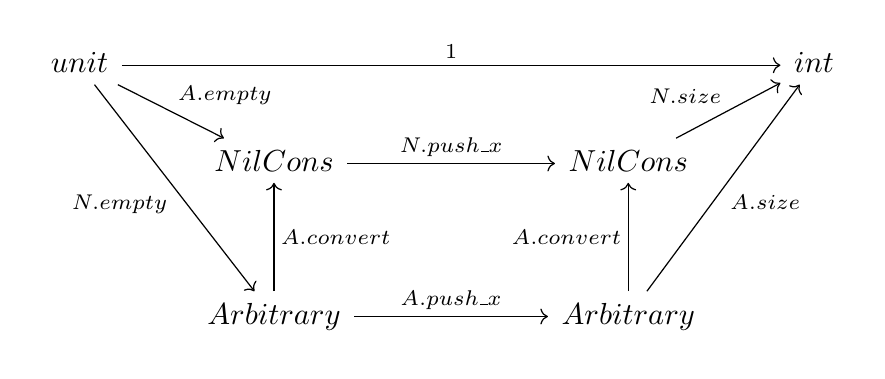
\begin{tikzpicture}
      % include tikzcd in a tikz node so that I can scale it.
      % yes, this is a ridiculous hack
      \node[scale=1.1] (a) at (0, 0){
      \begin{tikzcd}
        \code{unit} \arrow{dr}{\code{A.empty}} \arrow[swap]{dddr}{\code{N.empty}} \arrow{rrr}{\code{1}}& &[4em] & \code{int} \\
        & \code{NilCons} \arrow{r}{\code{N.push \_ x}} &[4em] \code{NilCons} \arrow{ur}{\code{N.size}} & \\
        & &[4em] & \\
        & \code{Arbitrary} \arrow[swap]{uu}{\code{A.convert}}  \arrow{r}{\code{A.push \_ x}} &[4em] \code{Arbitrary} \arrow{uu}{\code{A.convert}} \arrow[swap]{uuur}{\code{A.size}} &
      \end{tikzcd}
      };
    \end{tikzpicture}
    \caption{A commutative diagram demonstrating that \code{A.size (A.push x A.empty) = 1}, given that \code{N.size (N.push x N.empty) = 1} and that \code{A} and \code{N} commute. For simplicity, \code{1}, \code{N.empty}, and \code{A.empty} are treated as functions taking a \code{unit} argument.}
  \end{figure}

  \noindent This transference of correctness properties from the canonical implementation to arbitrary commuting implementations is valuable for two reasons. First, it allows us to extract properties that complicated implementations satisfy by only proving these properties for simple implementations. Second, it provides flexibility in the face of unsound correctness properties. Suppose an abstract type's collection of correctness properties is found to be unsound, and we revise the collection so that it becomes sound. Normally, we would need to prove the properties in the new collection for every implementation to ensure that every implementation is correct. With commutativity, we only need to prove this new collection of properties for the simple implementation, and these properties will transfer to every other implementation ``for free''.

  \subsection{Formalizing Commutativity}

  \noindent We will now formalize what it means for expressions to commute. Let \code{Ic<T1, ..., Tk>} and \code{Ia<T1, ..., Tk>} be canonical and arbitrary implementations of an abstract type, respectively. Let \code{convert : Ia<T1, ..., Tk> -> Ic<T1, ..., Tk>} be a conversion function from the arbitrary implementation to the canonical implementation. Two expressions \code{e'} and \code{e} commute over \code{convert}, denoted $\commutes{\code{e'}}{\code{e}}$, according to the following rules:

  \begin{figure}[H]
    \centering
    \begin{mathpar}
      \inferrule*{
        \code{convert e' = e}
      }{
        \commutes{\typinl{e'}{\code{Ia<}\tau_1, \dots, \tau_k\code{>}}}{\typinl{e}{\code{Ic<}\tau_1, \dots, \tau_k\code{>}}}
      }

      \inferrule*{
        \code{e' = e}\ \ \ \ \tau\ \text{does not contain}\ \code{Ia}\ \text{or}\ \code{Ic}
      }{
        \commutes{\typinl{e'}{\tau}}{\typinl{e}{\tau}}
      }

      \inferrule*[Left=Product]{
        \code{e' = (e1', e2')}\ \ \ \ \code{e = (e1, e2)}\ \ \ \ \commutes{\typinl{e1'}{\tau'_1}}{\typinl{e1}{\tau_1}}\ \ \ \ \commutes{\typinl{e2'}{\tau'_2}}{\typinl{e2}{\tau_2}}
      }{
        \commutes{\typinl{e'}{\tau'_1 \times \tau'_2}}{\typinl{e}{\tau_1 \times \tau_2}}
      }

      \inferrule*[Left=Function]{
        \forall\ \code{e'}\ \code{e},\  \commutes{\typinl{e'}{\tau'_1}}{\typinl{e}{\tau_1}} \implies \commutes{\typinl{f' e'}{\tau'_2}}{\typinl{f e}{\tau_2}}
      }{
        \commutes{\typinl{f'}{\tau'_1 \rightarrow \tau'_2}}{\typinl{f}{\tau_1 \rightarrow \tau_2}}
      }

      \inferrule*[Left=TaggedSum]{
        \code{e' = Ci ei'} \ \ \ \ \code{e = Ci ei} \ \ \ \ \commutes{\typinl{ei'}{\tau'_i}}{\typinl{e_i}{\tau_i}}
      }{
        \commutes{\typinl{e'}{\code{C1 of}\ \tau'_1\ \code{\|...\| Ck of}\ \tau'_k}}{\typinl{e}{{\code{C1 of}\ \tau_1\ \code{\|...\| Ck of}\ \tau_k}}}
      }
    \end{mathpar}
    \caption{Inference rules for expression commutativity, with product, function, and tagged sum types. Commutativity can also be extended to other typing constructs.}
  \end{figure}

  \noindent Arbitrary implementation \code{Ia} and canonical implementation \code{Ic} commute if and only if for each provided value \code{v}, $\commutes{\code{Ia.v}}{\code{Ic.v}}$. As an example, let's look at what it means for \code{ArbitraryLifoStack.push} and \code{NilConsLifoStack.push} to commute:

  \begin{figure}[H]
  \begin{mathpar}
    \inferrule*{
      \forall\ \code{l'}\ \code{l},\ \ \ \
      \inferrule*{
        \code{A.convert l' = l}
      }{
        \commutes{\typinl{l'}{\code{A<T>}}}{\typinl{l}{\code{N<T>}}}
      }
      \implies
      \inferrule*{
        \ddots \textit{(see below)} \iddots
      }{
        \commutes{\typinl{A.push l'}{\code{T} \rightarrow \code{A<T>}}}{\typinl{N.push l}{\code{T} \rightarrow \code{N<T>}}}
      }
    }{
      \commutes{\typinl{A.push}{\code{A<T>} \rightarrow \code{T} \rightarrow \code{A<T>}}}{\typinl{N.push}{\code{N<T>} \rightarrow \code{T} \rightarrow \code{N<T>}}}
    }

    \inferrule*{
      \forall\ \code{x'}\ \code{x}, \ \ \ \
      \inferrule*{
        \code{x' = x}
      }{
        \commutes{\typinl{x'}{\code{T}}}{\typinl{x}{\code{T}}}
      }
      \implies
      \inferrule*{
        \code{A.convert (A.push l' x') = N.push l x}
      }{
        \commutes{\typinl{A.push l' x'}{\code{A<T>}}}{\typinl{N.push l x}{\code{N<T>}}}
      }
      %\commutes{\typinl{A.push l' x'}{\code{A<T>}}}{\typinl{N.push l x}{\code{N<T>}}}
    }{
      \commutes{\typinl{A.push l'}{\code{T} \rightarrow \code{A<T>}}}{\typinl{N.push l}{\code{T} \rightarrow \code{N<T>}}}
    }
  \end{mathpar}
  \caption{Formal derivation of \code{A.push} and \code{N.push} commuting}
  \end{figure}

  \noindent Putting this together gives us:

  \begin{align*}
    & \forall\  \code{l' l x' x},\ \code{A.convert l' = l} \implies \\
    & \hspace{7.5 em} \code{x' = x} \implies \code{A.convert (A.push l' x') = N.push l x} \\
    \equiv\  & \forall\ \code{l x},\ \code{A.convert (A.push l x) = N.push (A.convert l) x}
  \end{align*}

  \noindent which is exactly the commutativity property listed above.

\section{Instantiations}

  To explore employing the commutativity paradigm in practice, I instantiated it in two abstract types using the Coq proof assistant: one abstract type for natural numbers, and another abstract type for arrays. All of the code can be found in a public Github repository (\href{https://github.com/ethantkoenig/CS-4860-Project}{\underline{link here}}).

\subsection{Instance 1: Natural Numbers}

  The standard implementation of the natural numbers in Coq is based on a unary representation. It is easy to prove properties about the natural numbers with this simple and elegant representation. However, the obvious downside of this implementation is its glaring inefficiency. In response to this inefficiency, more efficient implementations of the natural numbers have been added to Coq. In particular, the \code{BinNums} library offers a binary implementation of the natural numbers.

  \bigskip

  \noindent Any program that uses the natural numbers should not depend on how the natural numbers are implemented; instead, the program should only rely on the existence of particular values, such as zero, successor and addition, and properties that these values satisfy. This means that users of natural numbers could use an abstract type of natural numbers, as opposed to one particular implementation.

  \bigskip

  \noindent I wrote an abstract type for natural numbers using Coq's module system, and wrote multiple implementations of this abstract type using the commutativity paradigm:

  \begin{itemize}
    \item \code{NatInterface:} a module type which lists the values that a natural numbers implementation must provide
    \item \code{CanonicalNatImpl:} an implementation of \code{NatInterface} using the standard unary representation
    \item \code{CommutingNatInterface}: a module type extending \code{NatInterface} which introduces a \code{convert} value. It requires every provided value to commute with the corresponding \code{CanonicalNatImpl} value over \code{convert}. It also requires \code{convert} to be injective, which makes future proofs much cleaner.
    \item \code{CommutingCanonicalNatImpl:} an implementation of \code{CommutingNatInterface} using \code{CanonicalNatImpl}. Its \code{convert} value is the identity function, and all commutativity properties hold trivially.
    \item \code{VerifiedNatInterface}: a module type extending \code{CommutingNatInterface}, which includes a (possibly non-exhaustive) list of properties that a correct implementation of the natural numbers should satisfy.
    \item \code{VerifiedCommutingNatImpl}: a functor which accepts as an argument an implementation of \code{CommutingNatInterface}, and produces a corresponding implementation of \code{VerifiedNatInterface}
    \item \code{BinaryNatImpl}: an implementation of \code{CommutatingNatInterface} that uses \code{BinNums}'s binary representation.
  \end{itemize}

  \noindent In particular, the \code{VerifiedCommutingNatImpl} functor proves correctness properties for an arbitrary implementation of \code{CommutingNatImpl} using only the definitions in \code{CanonicalNatImpl} and proof that the commuting implementation does in fact commute.

\subsection{Instance 2: Naturally-Indexed Arrays}

  In addition to developing commutative implementations of abstract types, I also wanted instantiate a client's use of commutative implementations. To achieve this, I created an abstract type for arrays indexed by the natural numbers. Instead of relying upon a particular implementation of the natural numbers, the interface takes as an argument an implementation of \code{VerifiedNatInterface} to use as indices:

  \begin{itemize}
    \item \code{ArrayInterface}: a module type listing the values that an array implementation must provide. Takes an implementation of \code{VerifiedNatInterface} as an argument, which is used for the arrays' indices.
    \item \code{CanonicalArrayImpl}: an implementation of \code{ArrayInterface} using nil-cons lists.
    \item \code{CommutingArrayInterface}: a module type extending \code{ArrayInterface} which introduces a \code{convert} value. It requires every provided value to commute with the corresponding \code{CanonicalArrayImpl} value over \code{convert}.
    \item \code{CommutingCanonicalArrayImpl}: an implementation of \code{CommutingArrayInterface} using \code{CanonicalArrayImpl}. Its \code{convert} value is the identity function, and all of the commutativity properties hold trivially.
    \item \code{VerifiedArrayInterace}: an extension of \code{CommutingArrayInterface} which includes a (non-exhaustive) list of properties that a correct array implementation should satisfy.
    \item \code{VerifiedCommutingArrayImpl}: a functor which accept as an argument an implementation of \code{CommutatingArrayInterface}, and produces a corresponding implementation of \code{VerifiedArrayInterface}.
    \item \code{TreeArrayImpl}: an implementation of \code{CommutatingArrayInterface} using binary trees.
  \end{itemize}

  \noindent Similar to \code{VerifiedCommutingNatImpl}, the \code{VerifiedCommutingArrayImpl} functor proves correctness properties for an arbitrary implementation of \code{CommutingArrayInterface} using only the definitions in \code{CanonicalArrayImpl}, and proof that the commuting implementation does in fact commute.

\section{Conclusion}

  % course relevance

  With all of this said, how do commuting implementations of abstract types build on top of what we've covered in CS 4860? The main ways in which this project relates to the course are its use of dependent types to formulate commutativity properties in first-order-logic, its use of refinement logic to prove these properties, and its use of constructive type theory as a foundation of computation.

  \bigskip

  \noindent The commutativity properties for abstract type implementations are stated using first order logic. When these properties are expressed as types, via the Curry-Howard isomorphism, they are dependent types. In the Coq instantiations of the commutativity paradigm, commutativity properties are expressed as dependently-typed values that commuting implementations must provide.

  \bigskip

  \noindent Additionally, I used refinement logic to prove these commutativity properties, and to prove that commutativity properties in turn imply more general properties. The refinement logics supported by proof assistants like Coq and NuPRL are built upon the refinement logic for first order logic that we covered in lecture.

  \bigskip

  \noindent Finally, the commutativity paradigm, and its instantiations in Coq, are founded upon constructive type theory. In particular, the distinction between canonical and non-canonical values that is made in constructive type theory shows up in commutativity properties. Every commutativity property contains subterms of the form \code{e1 = e2}, where \code{e1} and \code{e2} are expressions. The proposition \code{e1 = e2} is not asserting that \code{e1} and \code{e2} are syntactically equivalent, but instead that they reduce to the same canonical value.

  \bigskip

  % practical interest

  \noindent In addition to pertaining to the material we covered in CS 4860, commuting implementations also are of practical interest. The most immediate application of logic to computer science is software verification. Proof assistants and other advances in formal methods have enabled the verification of increasingly sophisticated software, from kernels to compilers. Meanwhile, software systems have come to underlie finance, defense, medicine, and many of the world's most critical institutions. These increasingly high-stakes roles create a pressing demand for error-free systems.

  \bigskip

  \noindent Unfortunately, proving software correct remains an expensive endeavor, and for this reason the vast majority of software has not been formally verified. Finding less expensive methods for verification that still provide formal guarantees will enable wider adoption of software verification. The commutativity paradigm is a step in this direction, as it allows correctness properties proven for a simple implementation of an abstract type to be extended to arbitrarily complex implementations at no additional cost. It is my hope that this work becomes a small step towards making the world's software more reliable.

\section{Acknowledgments}

  Thanks to Professor Robert Constable for teaching the logic that underlies this work in CS 4860.

  \bigskip

  \noindent Thanks to Adam Chlipala and Michael Nahas for their tutorials of Coq, which helped me become familiar with the proof assistant.

  \bigskip

  \noindent Thanks to many unnamed StackOverflow contributors whose \LaTeX \ advice made this report's formatting much more pleasant and digestible than it would have been otherwise.

\begin{thebibliography}{9}
  \bibitem{bib:cpdt} A. Chlipala, \textit{Certified programming with dependent types: A pragmatic introduction to the Coq proof assistant}. Cambridge, MA: The MIT Press, 2014.
  \bibitem{bib:cs4860} R. Constable, ``CS 4860: Applied Logic,'' 2016.
  \bibitem{bib:nahas} M. Nahas, ``A tutorial by Mike Nahas,'' in \textit{The Coq Proof Assistant}, 2014. [Online]. Available: https://coq.inria.fr/tutorial-nahas. Accessed: 2016.
  \bibitem{bib:smull} R. M. Smullyan, \textit{First-order logic}. New York: Dover Publications, 2003.

\end{thebibliography}

\end{document}

